%&program=pdflatex
%&encoding=UTF-8 Unicode
\documentclass[a4paper]{llncs}
\usepackage{llncsdoc}

%% Deutsche Anpassungen %%%%%%%%%%%%%%%%%%%%%%%%%%%%%%%%%%%%%
\usepackage[ngerman]{babel}
\usepackage[T1]{fontenc}
\usepackage[utf8]{inputenc}
%\usepackage{fontspec}
%\setromanfont[Mapping=tex-text,Alternate=1,Ligatures={Common,Diphthong}]{Palatino} 

% Mateh
\usepackage{amsmath}
\usepackage{amssymb}

% Paket für Graphiken
\usepackage[pdftex]{graphicx}

%\Paket für Hyperlinks
\usepackage[
bookmarks=true,
bookmarksopen=true,
bookmarksnumbered=true,
breaklinks=true,
colorlinks=true,
linkcolor=black,
anchorcolor=black,
citecolor=black,
filecolor=black,
menucolor=black,
pagecolor=black,
urlcolor=black
]{hyperref}

\begin{document}

\title{Clustering of DBPedia Subjects}
\subtitle{Seminar Map/Reduce Algorithms on Hadoop}
\author{Robert Pfeiffer, Tobias Schmidt}
\institute{Fachgebiet Informationssysteme\\Hasso-Plattner-Institut für Softwaresystemtechnik\\Prof.-Dr.-Helmert-Str. 2-3\\14482 Potsdam, Deutschland\\31. August 2009}

\maketitle

\begin{abstract}
TODO\\
wenn alles fertig ist\\
werden es mal 3 Zeilen?
\end{abstract}

\section{Einleitung}
Mit der fortschreitenden Nutzung der Computertechnik in allen Lebensbereichen steigt auch das zu bearbeitende Datenvolumen stetig an. Damit auf immer größeren Datenmengen weiterhin effizient Berechnungen ausgeführt werden können, wurde von Google\footnote{\url{http://www.google.com/}} ein Berechnungsmodell namens MapReduce entwickelt. Mit dieser Architektur ist es möglich, Berechnungen auf mehrere Computer zu verteilen und parallel ablaufen zu lassen.

Im Seminar \emph{Map/Reduce Algorithms on Hadoop}\footnote{\url{http://www.hpi.uni-potsdam.de/naumann/lehre/ss_09/mapreduce_algorithms_on_hadoop.html}} haben wir uns mit dem, in Java implementierem, MapReduce-Framework \emph{Hadoop}\footnote{\url{http://hadoop.apache.org/}} auseinandergesetzt und einen Algorithmus implementiert, der eine Menge von Objekten anhand ihrer Ähnlichkeit gruppiert.

\section{Grundlagen}

\subsection{MapReduce}
MapReduce ist ein Programmiermodell, welches erstmals 2004 vorgestellt wurde \cite{DG04} und Prinzipien funktionaler Programmierung aufgreift. 
Der MapReduce Ansatz besteht im Allgemeinen aus zwei Funktionen: \emph{Map} und \emph{Reduce}. In der Map-Funktion wird ein Problem in mehrere Teilprobleme zerlegt, die idealerweise parallel und unabhängig voneinander ausgeführt werden.
Anschließend werden die Ergebnisse der Teilprobleme in der Reduce-Funktion wieder zu einem Gesamtergebnis zusammengesetzt.

Die Map-Funktion erwartet als Eingabe Schlüssel-Wert-Paare und gibt neue Schlüssel-Wert-Paare als Ergebnis aus.
Die Reduce-Funktion erhält als Eingabe einen Schlüssel und alle dazugehörigen Werte.
Diese Werte werden je nach vorgegebener Berechnung zusammengeführt und dem Schlüssel zugeordnet.
Die Reduce gibt anschließend wiederum Schlüssel-Wert-Paare aus.

\subsection{Hadoop TODO}
Hadoop stellt ein verteiltes Dateisystem bereit.
%Nodes
%HDFS
%Yahoo,Apache
Das Hadoop MapReduce-Framework übernimmt die Zerteilung der Eingabedatei und generiert aus den einzelnen Teilen sogenannte Maptasks.
Die einzelnen Rechner im Hadoop-Cluster bearbeiten anschließend diese Maptasks.
Für jedes Schlüssel-Wert-Paar wird die Map-Funktion aufgerufen. Der Task-Tracker überwacht den Fortschritt auf den Nodes und teilt ihnen bei Bedarf weitere Tasks zu. Dabei werden Tasks bevorzugt auf den Rechnern ausgeführt, die bereits die dazu nötigen Daten haben, weil sie den entsprechenden Teil des verteilten Dateisystems verwalten.

Der Job-Tracker überwacht den Gesamtfortschritt eines MapReduce-Schrittes, generiert die Map- und Reduce-Tasks und kümmert sich um die Ein- und Ausgabe.

\subsection{Die Daten}
Die Datenmenge, die uns zur Verfügung gestellt wurde, sind Ressourcen aus der \emph{DBPedia}\footnote{\url{http://dbpedia.org/}}.
Das \emph{DBPedia}-Projekt extrahiert Informationen aus der Online-Enzyklopädie \emph{Wikipedia}\footnote{\url{http://www.wikipedia.org/}}, bereitet diese auf und stellt diese strukturiert zur freien Verfügung.
Einträge der \emph{DBPedia} entsprechen damit weitesgehend Artikeln der \emph{Wikipedia}.
Als Hauptquelle für Informationen in der DBPedia sind die Infoboxen zu nennen, die in vielen Artikeln auf der rechten Seite existieren.

Die Daten werden als RDF-Tripel der Form $(Subject, Attribut, Wert)$ in der DBPedia gehalten (z.B. $(Berlin, populationTotal, 3429300)$).
Die ca. 44.000 verschiedenen Attribute der DBPedia sind in eine Ontologie eingeordnet.
Da alle Ressourcen aus dieser Ontologie stammen, kann man davon ausgehen, dass gleiche Attribute die gleiche Semantik haben. Dadurch lassen sich aus dem Gruppieren der Subjekte nach ähnlichen Attributmengen möglicherweise semantische Rückschlüsse ziehen.

\subsection{Clustering}
Algorithmen, beziehungsweise Verfahren, die eine Menge von Objekten zu Gruppen (Cluster) mit jeweils ähnlichen Eigenschaften zusammenfassen, bezeichnet man als Clusteranalyseverfahren.
Es gibt eine ganze Reihe von unterschiedlichen Ansätzen zur Analyse, die alle unterschiedliche Vor- und Nachteile haben.
Grundsätzlich unterscheidet man zwischen partitionierenden und hierarchischen Analyseverfahren.

Für viele Clusterverfahren wird ein Abstandsmaß benötigt. Dieses gibt für zwei Objekte einen Wert zurück, der angibt, wie weit die beiden Objekte voneinander entfernt sind. Kleinere Werte beschreiben üblicherweise geringere Abstände. Es gibt verschiedene Abstandsmaße, die für unterschiedlichen Daten unterschiedlich gute Ergebnisse liefern. Als Beispiele sind das \emph{Euklidische Abstandsmaß} und die \emph{Jaccard-Distanz} zu nennen.

\subsection{k-Means}
Wir haben das partitionierende Clusteranalyseverfahren \emph{k-Means}\footnote{\url{http://de.wikipedia.org/wiki/K-Means-Algorithmus}} angewendet. % vielleicht Literatur statt weblink
\emph{k-Means} zeichnet sich durch seine hohe Geschwindigkeit aus, liefert jedoch nicht zwingend die optimale Lösung. Desweiteren muss man bei \emph{k-Means} die Anzahl der gewünschten Cluster im Vorfeld vorgeben.

Zu Beginn des Algorithmus wählt man zufällig die gewünschte Anzahl von Clustern aus der Objektmenge aus. Diese Objekte bilden die initialen Clusterzentren. Aus der zufälligen Auswahl der Clusterzentren ergibt sich die Konsequenz, dass bei verschiedenen Programmdurchläufen mit gleichen Eingabedateien unterschiedliche Cluster berechnet werden können. Nach der Wahl der Clusterzentren beginnt der iterative Teil des Algorithmus.

Für jedes Objekt wird mit Hilfe des Abstandsmaßes der Abstand zu jedem Clusterzentrum berechnet. Anschließend wird das Objekt demjenigen Cluster zugeordnet, zu dessen Clusterzentrum es den geringsten Abstand aufweist.
Nachdem alle Objekte einem Cluster zugeordnet worden sind, wird das neue Clusterzentrum bestimmt, indem der Schwerpunkt aller dem Cluster zugeordneten Objekte berechnet wird.

Dieser Vorgang wird solange wiederholt, bis nach einer Iteration kein Objekt mehr einem anderen Clusterzentrum zugeordnet wird. Alternativ kann auch eine prozentuale Schranke festgelegt werden (zum Beispiel: wiederhole bis weniger als 2\% der Objekte einem anderen Cluster zugeordnet werden).

\subsection{Jaccard-Distanz}
Die Jaccard-Distanz ist ein Abstandsmaß, dass die Ähnlichkeit zwischen Mengen angibt. Dabei sind zwei Mengen einander ähnlicher, je mehr Elemente sie gemeinsam haben. Die Jaccard-Distanz von einer Menge zu sich selbst ist Null.

%Die Jaccard-Distanz basiert auf dem Jaccard-Index, dem Quotienten aus Schnitt- und Vereinigungsmenge zweier Mengen.

$$J_{\delta}(A,B) = %1 - J(A,B) = 
{ { |A \cup B| - |A \cap B| } \over |A \cup B| }$$

Ein Vorteil der Jaccard-Distanz gegenüber dem euklidischen Abstandsmaß ist, dass Elemente, die in den jeweiligen Mengen enthalten sind, stärker berücksichtigt werden, als nicht enthaltene Elemente. Beim Euklidischen Abstand beeinflussen Elemente, die in beiden Mengen fehlen oder vorhanden sind, das Abstandsmaß gleich.

\subsection{Fuzzy-Mengen}
Da die Clusterzentren gemittelte Werte enthalten, können sie nicht wie die Subjekte als einfache Mengen dargestellt werden.
Stattdessen werden Fuzzy-Mengen benutzt. Bei Fuzzy-Mengen kann ein Element zu einem gewissen Grad zwischen 0 und 1 enthalten sein.
Dies wird durch die Funktion $\mu : M \times E \rightarrow [0,1] $ beschrieben. Dabei bedeutet $m(A,e) = 0$ soviel wie $ e \not\in A $ und $m(A,e) = 1$ entspricht $ e \in A $ aus der normalen Mengenlehre.

Die Identitäten für Schnitt- Vereinigungsmengen in der Mengenlehre \begin{align*}e \in (A \cap B) = (e \in A) \wedge (e \in B)
	\\ e \in (A \cup B) = (e \in A) \vee (e \in B) \end{align*} lauten für Fuzzy-Mengen  \begin{align*}\mu(e, A \cap B) = min(\mu(e, A), \mu(e, B))\\ \mu(e, A \cup B) = max(\mu(e, A), \mu(e, B))  \end{align*}.

Damit lässt sich der Jaccard-Index numerisch auf folgende Weise berechnen:

$P$ sei die Menge aller möglichen Attribute.
$$J_{\delta}(A,B) = \frac{\sum\limits_{p \in P}max\bigl(\mu(p, A)\mu(p, B)\bigr) - min\bigl(\mu(p, A),\mu(p, B))\bigr)}{\sum\limits_{p \in P}max\bigl(\mu(p, A),\mu(p, B))\bigr)}$$

\section{Implementation}

\subsection{Datenformat}
%- Problem: Daten sind große Matrizen\\
%- Vorteile:\\
%    - Hadoop Format, dadurch gibt es bereits ein Interface und Hadoop kann den Input splitten\\
%    - komprimiert\\
%- Nachteile:\\
%    - kodiertes Format, daher für Menschen nicht lesbar\\
 %   - keine Information über die Gesamtgröße
Die Eingabedateien enthalten die Subjekte in einem Binärformat. Dabei wird jedes Subjekt durch ein Array von Bits repräsentiert, wobei die Stelle im Array immer ein Attribut repräsentiert. Wenn an einer Stelle ein 1-Bit steht, dann besitzt die Ressource das Attribut.

\subsection{Sequence Files}
Sequence Files sind ein Dateiformat von Hadoop. Sie enthalten Schlüssel-Wert-Paare von serialisierten Objekten. Die Schlüssel-Wert-Paare in einer sequence-File müssen jeweils vom gleichen Typ sein 
Die meisten Hadoop-Klassen sind in Sequence Files serialisierbar.
Das Hadoop-Framework enthält neben dem Text-InputFormat unter anderem auch ein InputFormat für Sequence Files, sowie die Möglichkeit, Sequence Files aufzusplitten um sie auf verschiedene Map-Tasks zu verteilen.

\subsection{Generierung der Clusterzentren}
Das erste Problem bei der Implementierung des \emph{k-Means} Algorithmus stellte die Generierung der initialen Clusterzentren dar. Im Hadoop-Framework werden eine Map- und eine Reduce-Funktion zu einem Job zusammengefasst und es ist möglich, in einem Programm mehrere Jobs hintereinander auszuführen. Dadurch bestand eine Möglichkeit darin, mittels eines Jobs die Zentren zu generieren und mit Hilfe eines zweiten Jobtyps den iterativen Teil des Algorithmus auszuführen. Die zweite von uns erarbeitete Idee war, die Clusterzentren vor dem Starten des Hadoop-Programmes separat zu generieren und als weiteren Eingabeparameter mitzuliefern. Wir haben uns für das zweite Verfahren entschieden, da es zum einen zu diesem Zeitpunkt für uns leichter zu implementieren war und zum anderen durch die einmalige Generierung einen Geschwindigkeitsvorteil darstellte. Für eine finale Version des Programms wäre es jedoch von Vorteil, wenn der Benutzer nicht selbst die Clusterzentren generieren müsste.

% hat auch Vorteile beim evaluieren

\subsection{Distributed Cache}
%- Problem: Verteilung der Centroids\\
%- Lösung mittels Distributed Cache\\
%- Vorteile: in Hadoop, synchrone Datenhaltung, wenig Overhead für die restlichen berechnungen\\
%- Nachteile: bricht das Map/Reduce Konzept\\
%- andere Möglichkeit: kartesisches Produkt

Um die Cluster in einer Iteration des \emph{k-Means}-Algorithmus neu zu bestimmen, muss der Abstand jedes Subjektes von jedem Zentrum berechnet werden. Die Eingabedaten müssen für die Verarbeitung mit MapReduce so aufgeteilt werden, dass dies möglich ist.

Anstatt das kartesische Produkt von Clusterzentren und Subjekten zu bilden und anschließend zu verteilen, wird eine Liste von Zentren den Mappern zu Beginn jeder Iteration als Parameter übergeben. Da die Anzahl der Cluster, und demzufolge auch die der Clusterzentren, viel kleiner als die Anzahl der Subjekte ist, bewirkt dieses Vorgehen einen sehr geringen Kommunikationsaufwand. Da im Map-Schritt alle Zentren bekannt sind, kann das nächste Zentrum, und damit die Clusterzugehörigkeit jedes Subjektes, bereits im Map-Schritt bestimmt werden. 

Parameter können nicht direkt an die Mapper übergeben werden, da die Job-Konfiguarion nicht die Mapper kennt, sondern nur deren Klassennamen. Die Mapper werden erst auf den Knoten erzeugt. Um den Mappern zusätzliche Parameter zu übergeben, werden deshalb zusätzliche Einträge in der Konfiguration sowie der \emph{Distributed Cache} verwendet. Der \emph{Distributed Cache} bietet die Möglichkeit, größere Datenmengen an die Knoten zu übermitteln, bevor der eigentliche MapReduce-Zyklus beginnt. Dazu werden die Dateien, die zum \emph{Distributed Cache} hinzugefügt wurden, vom HDFS in das lokale Dateisystem auf den Knoten kopiert. Im Gegensatz zum HDFS stellt der \emph{Distributed Cache} sicher, dass jeder Knoten alle Dateien vollständig erhält, bevor ein MapReduce-Zyklus beginnt.

Die Knoten können jederzeit auf die lokalen Dateien lesend zugreifen. In unserer Implementierung werden mit der Erzeugung der Mapper die Clusterzentren auf den Knoten ausgelesen und anschließend im Hauptspeicher gehalten.

\subsection{Berechnung der Cluster}
\label{sec:BerechnungDerCluster}
Nachdem die Clusterzentren mittels des \emph{Distributed Cache} auf die einzelnen Knoten verteilt wurden, beginnt die eigentliche Berechnung.
Der iterative Teil des \emph{k-Means}-Algorithmus lässt sich relativ leicht auf das MapReduce-Schema abbilden. Für jedes Subjekt wird eine Map-Funktion aufgerufen. 
Diese berechnet den Abstand des Subjektes zu jedem Clusterzentrum, welche mittels \emph{Distributed Cache} zur Verfügung stehen.

Für die Abstandsberechnung haben wir ein Interface \emph{Distance} eingeführt, welches unter anderem die Funktion \emph{between} bereitstellt.
Diese Funktion erwartet als Eingabe zwei Vektoren gleicher Länge und gibt eine reelle Zahl zurück, welche den Abstand zwischen den beiden Vektoren repräsentiert.
Wir haben mit dem \emph{Euklidischen Abstandsmaß} und der \emph{Jaccard Distance} zwei verschiedene Implementationen des Interfaces erstellt.
Dem Anwender ist es selbst überlassen, welche Implementation er verwenden möchte. Er kann dies durch die Konfigurationsdatei einstellen.

Das Resultat der Map-Funktion ist ein Schlüssel-Wert-Paar, bestehend aus dem Schlüssel des nächsten Clusterzentrums und dem Vektor des Subjektes.

Die Reduce-Phase beginnt, sobald für jedes Subjekt das nächste Clusterzentrum berechnet wurde.
Für jeden eindeutigen Schlüssel wird die Reduce-Funktion genau einmal gerufen. Als Wert wird eine Liste aller Vektoren übergeben, 
die diesem Clusterzentrum (sprich diesem Schlüssel) zugeordnet wurden. Um den neuen Schwerpunkt des Clusterzentrums zu berechnen,
wird erst die Summe aller Vektoren gebildet und diese anschließend durch die Anzahl der Vektoren dividiert.
Die Reduce-Funktion gibt anschließend ein Schlüssel-Wert-Paar mit dem Schlüssel des Clusters und dem neuen Schwerpunkt als Vektor zurück.

\subsection{Abbruch der Iteration}
Da der \emph{k-Means}-Algorithmus erst nach mehreren, im Vorfeld nicht genau bestimmbaren, Iterationen das gewünschte Ergebnis liefert,
muss der in \ref{sec:BerechnungDerCluster} beschriebene Prozess mehrmals ausgeführt werden.
% Allerdings genügt es nicht, nur den Job, der die beschriebenen Map- und Reduce-Funktionen enthält, erneut anzustoßen. Zuvor muss die Ausgabe der Reduce-Funktion, 
% welche die neu berechneten Clusterzentren enthält, in den \emph{Distributed Cache} verschoben werden, 
% um in der nächsten Iteration nicht mit den selben Daten erneut zu rechnen.
Nach der Definition von \emph{k-Means} wird dieser Zyklus beendet, sobald keine bzw. nur noch sehr wenige Subjekte einem anderen Cluster zugeordnet wurden.
Dies stellte sich bei unserer Implementation als Problem heraus, da aus Platz- und Geschwindigkeitsgründen keine Informationen über die Zuordnung von Subjekten zu Clustern gespeichert werden. Diese Informationen stehen nur zu Beginn des Reduce-Schrittes zur Verfügung, nicht aber nach Abschluss des Jobs.
Da das Mitführen der Zuordnungen sowie das dauerhafte Speichern sowohl die zwischen den einzelnen Knoten zu übertragenen Datenmengen stark erhöht,
als auch in einer komplexeren Programmstruktur gemündet hätte, entschieden wir uns gegen diese Lösung. 
Stattdessen berechnen wir den Fortschritt über die prozentuale Veränderung der Clusterzentren. Bevor die alten Clusterzentren im \emph{Distributed Cache} durch die neuen ersetzt werden, wird für jedes neu berechnete Clusterzentrum der Abstand zum alten Clusterzentrum berechnet. 
Die größtmögliche Entfernung von zwei Vektoren entspricht einer Veränderung von 100\%. Sinkt der Durchschnitt aller Veränderungen unter eine, vom Benutzer definierte, Schranke, so wird der Zyklus abgebrochen.

\section{Evaluierung}
Eingabegröße
\begin{figure}[!ht]
\centering
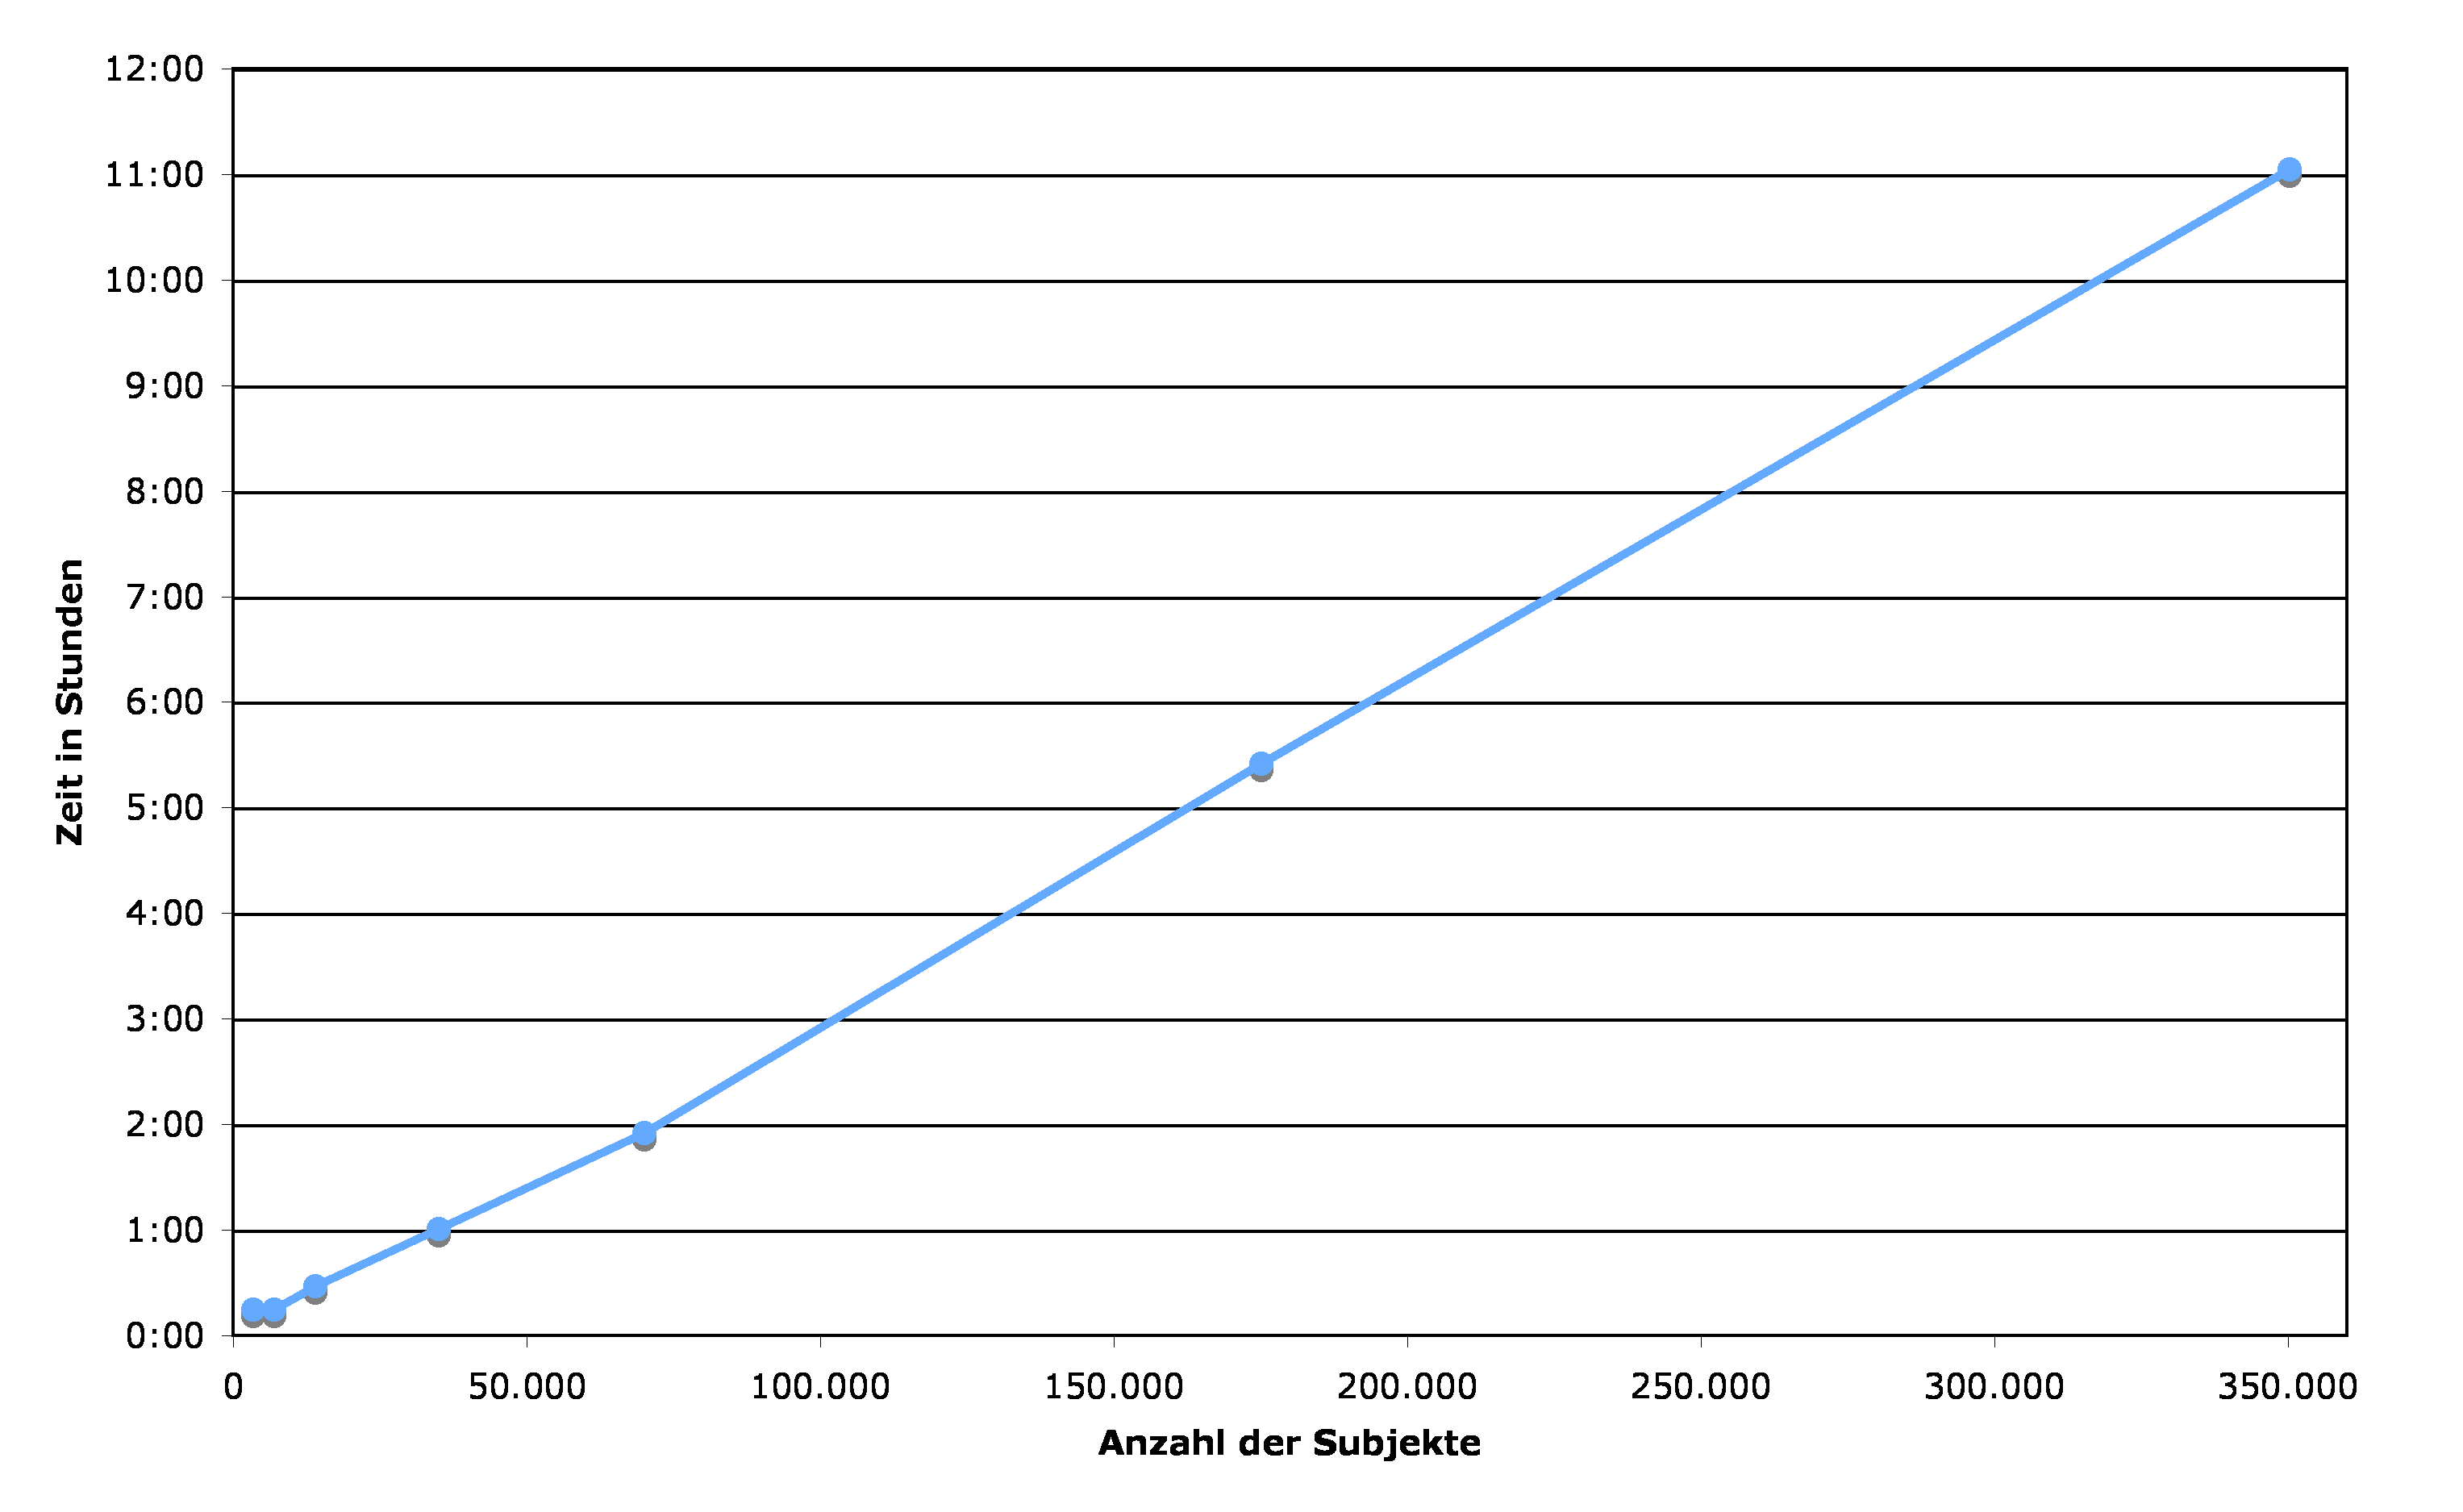
\includegraphics[width=0.99\textwidth]{charts/subjects.png}
\caption{Unterschiedliche Eingabegrößen}
\label{fig:subjects}
\end{figure}

Anzahl der Cluster
\begin{figure}[!ht]
\centering
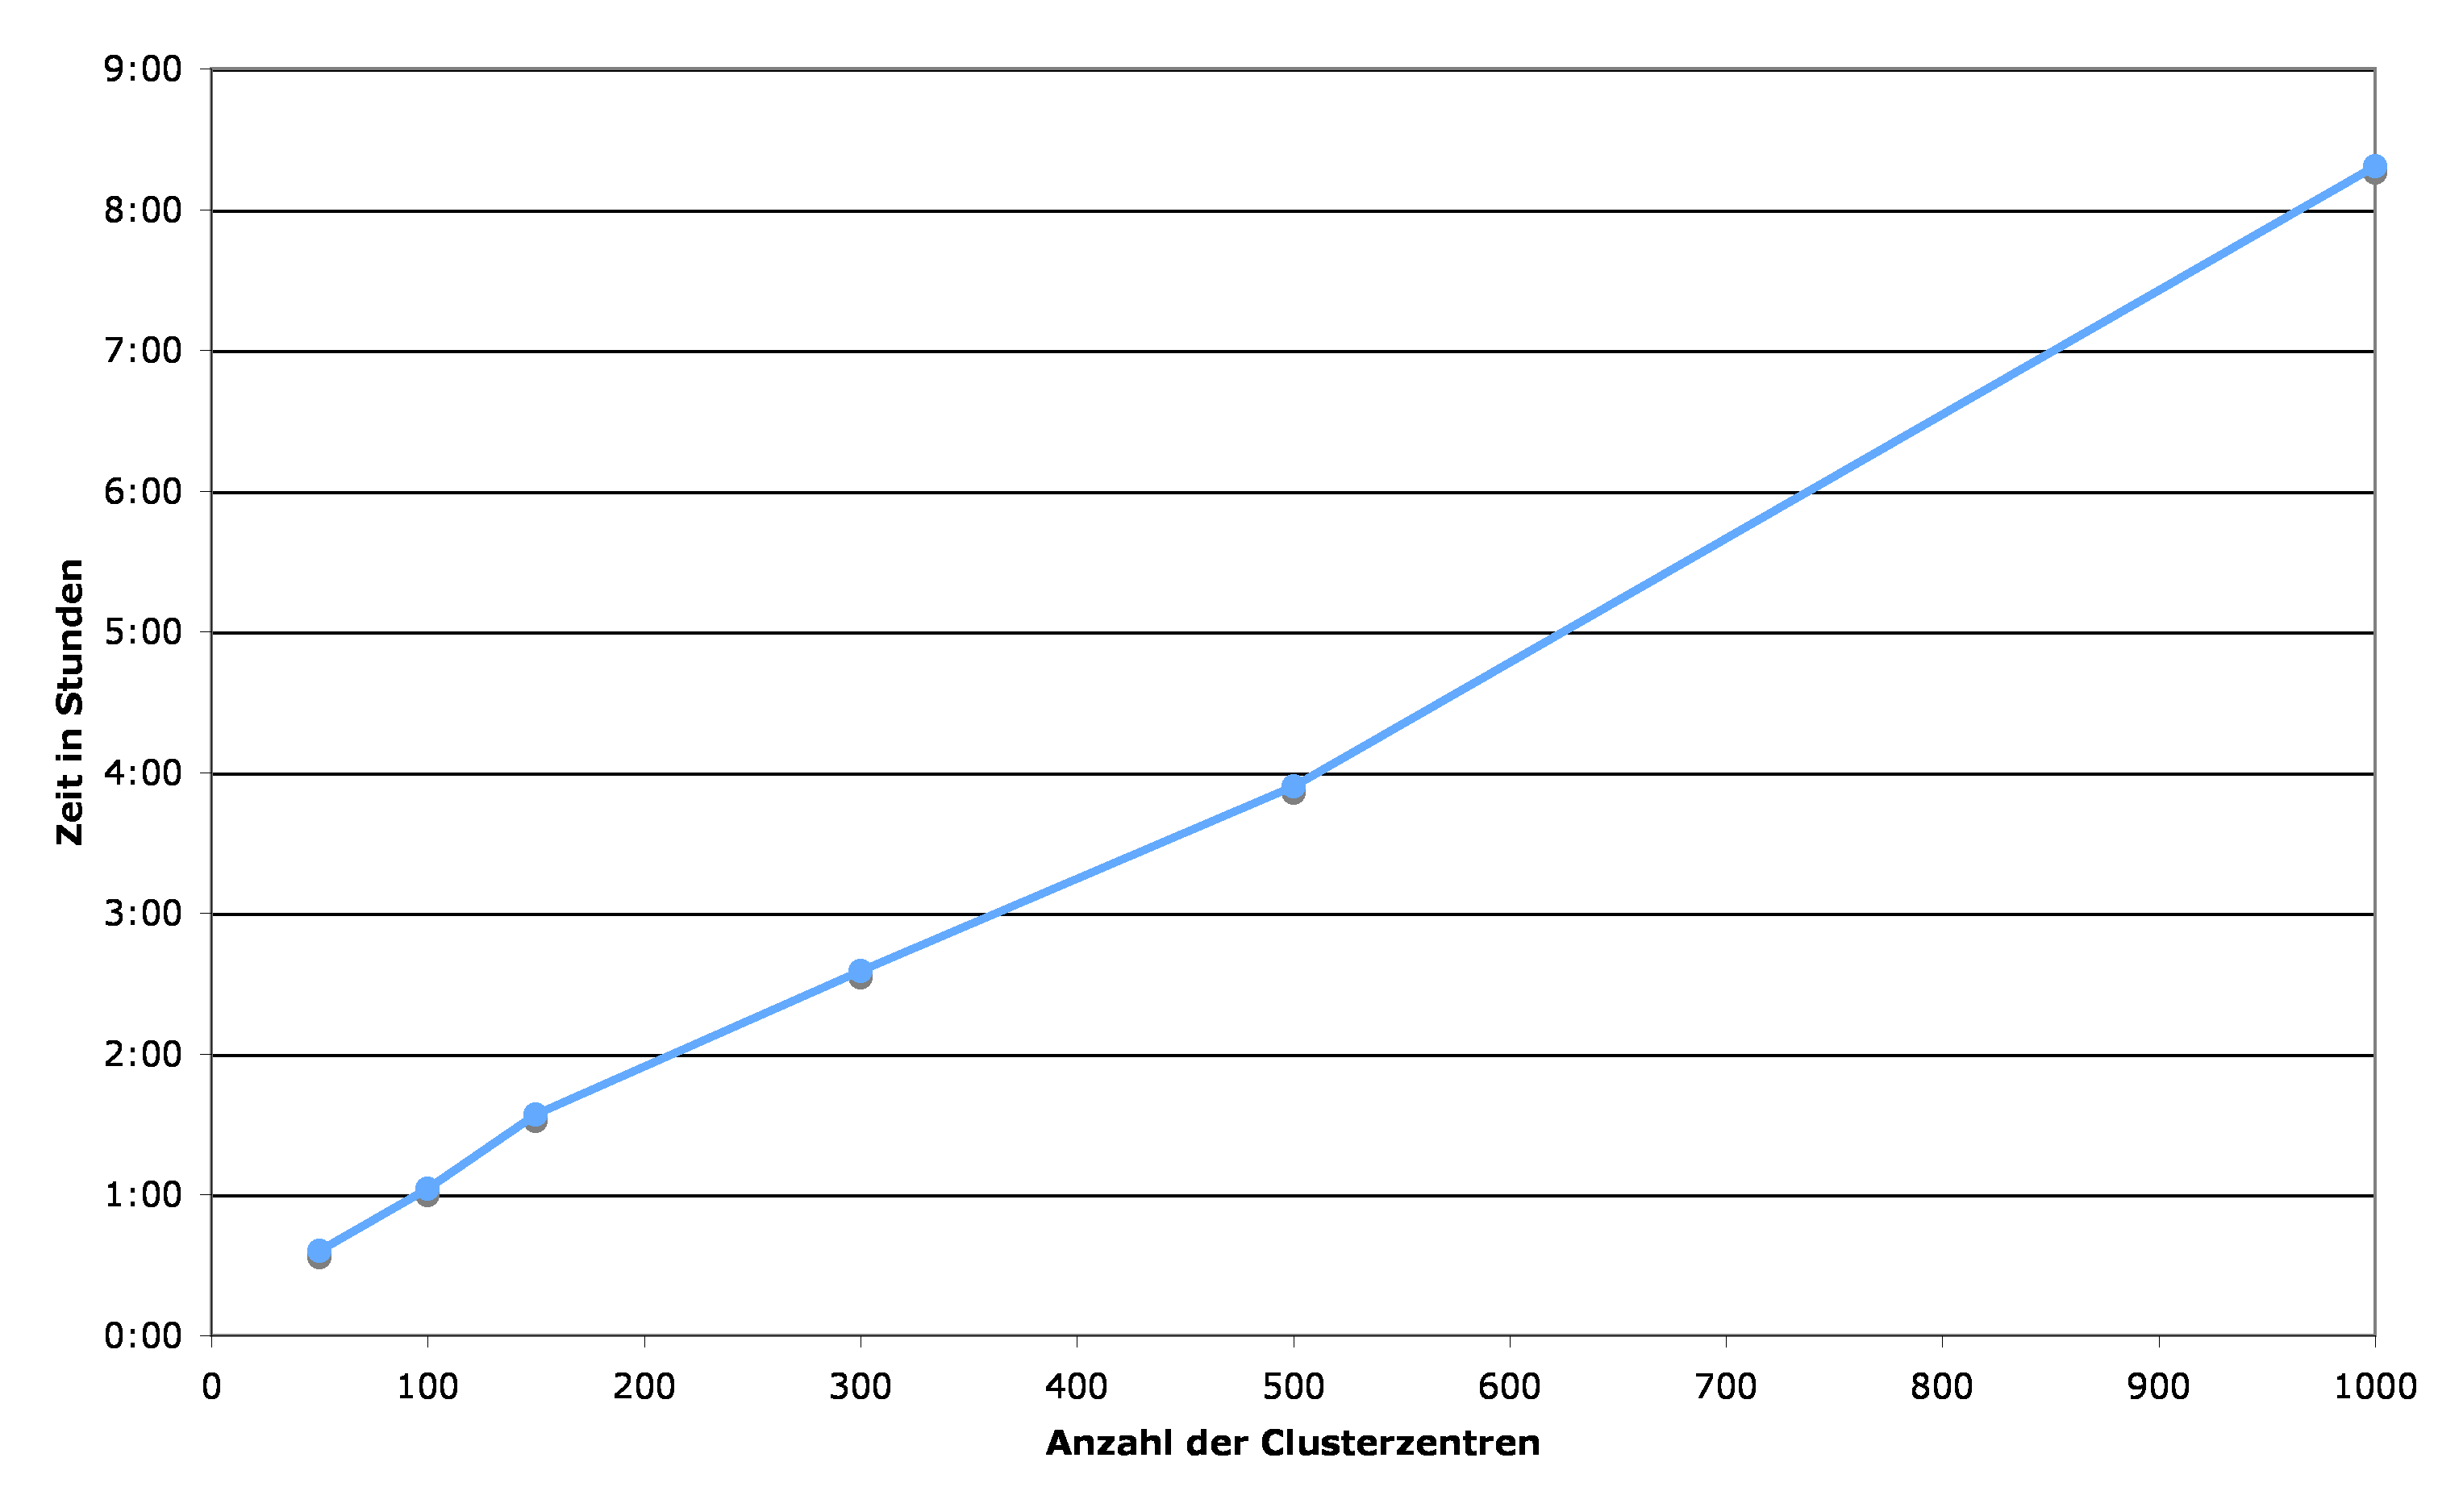
\includegraphics[width=0.99\textwidth]{charts/clustercenters.png}
\caption{Unterschiedliche Anzahl von Clusterzentren}
\label{fig:centers}
\end{figure}

Abbruch
\begin{figure}[!ht]
\centering
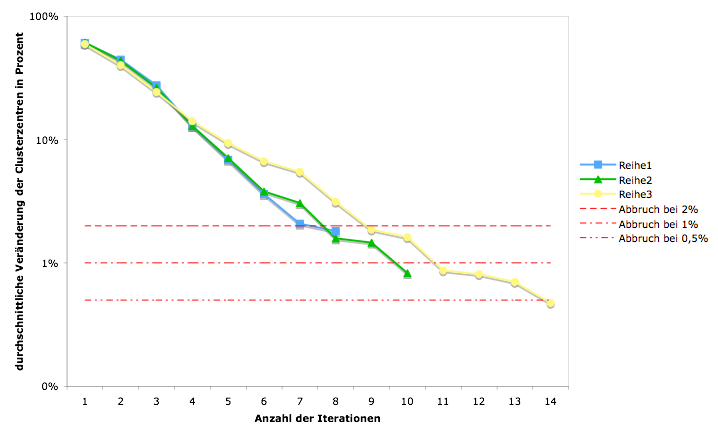
\includegraphics[width=0.99\textwidth]{charts/iterations_log.png}
\caption{Abbruch}
\label{fig:iterations}
\end{figure}

\section{Fazit}
- HDFS vs. lokales Dateisystem
TODO

\begin{thebibliography}{------------}

\bibitem[KI2008]{KI2008}
  Segaran, Toby.
  {\em Kollektive Intelligenz}.
  O'Reilly, 2008

\bibitem[DG04]{DG04}
  Dean, Jeffrey; Ghemawat, Sanjay.\\
  {\em MapReduce: Simplified Data Processing on Large Clusters}.\\
  San Francisco, CA, 2004
   
\end{thebibliography}

\end{document}
